%---------------------------PREAMBLE-------------------------------------------- %
\documentclass[9pt]{article}
% \documentclass[9pt]{amsart}
% \documentclass[9pt]{revtex4-2}


%------------------- PACKAGES 

\usepackage{graphicx}
	\graphicspath{ {plots/} }
\usepackage{caption}
\usepackage{epstopdf}
\usepackage{pdfpages}
\usepackage{array}
\usepackage{ulem}
\usepackage{amsfonts}
\usepackage{amssymb}
\usepackage{amsmath}
\usepackage{amsthm}
	\newtheorem{definition}{Definition}[section]
	\newtheorem*{remark}{Remark}
	\newtheorem{theorem}{Theorem}[section]
	\newtheorem{corollary}{Corollary}[theorem]
	\newtheorem{lemma}[theorem]{Lemma}
\usepackage{mathrsfs}
\usepackage{color}
\usepackage{float}
\usepackage{tikz}
\usetikzlibrary{arrows,%
                plotmarks,patterns}
\usepackage{pgfplots}
\pgfplotsset{compat=newest}
\usepgfplotslibrary{fillbetween}

\usepackage{enumerate}
\usepackage{array}
\usepackage{wrapfig}
\usepackage{enumitem}
\usepackage{bm}
\usepackage{booktabs}
\usepackage{siunitx}
\usepackage{authblk}
\usepackage{cancel}
\usepackage{listings}
\usepackage[utf8]{inputenc}

% \usepackage[table]{xcolor}

\usepackage[unicode,psdextra, colorlinks=true, linkcolor=black, citecolor=black, urlcolor=blue, breaklinks]{hyperref}[2012/08/13]


\setlength{\arrayrulewidth}{0.5mm}
% \setlength{\tabcolsep}{10pt}
\renewcommand{\arraystretch}{1.0}


%------------------ USEFULL MACROS ------------------%
%-- MISC
\newcommand{\comment}[1]{}                                % for adding an inline comment
\makeatletter 											  % This entire thing is for redefining *matrix environment in amsmath so that you can specify the line spacing in a matrix by  - \begin{pmatrix}[1.5]
\renewcommand*\env@matrix[1][\arraystretch]{%             
  \edef\arraystretch{#1}%
  \hskip -\arraycolsep
  \let\@ifnextchar\new@ifnextchar
  \array{*\c@MaxMatrixCols c}}
\makeatother

%-- DERIVATIVES
\newcommand{\der}[2]{\frac{\mathrm{d}#1}{\mathrm{d}#2}}          	 % first derivative
\newcommand{\dder}[2]{\frac{\mathrm{d}^{2}#1}{\mathrm{d}#2^{2}}}	 % second derivative
\newcommand{\nder}[3]{\frac{\mathrm{d}^{#3}#1}{\mathrm{d}#2^{#3}}}   % nth derivative
\newcommand{\pder}[2]{\frac{\partial #1}{\partial #2}}               % first partial derivative
\newcommand{\ppder}[2]{\frac{\partial^2 #1}{\partial {#2}^2}}        % second partial derivative
\newcommand{\npder}[3]{\frac{\partial^{#3} #1}{\partial {#2}^{#3}}}  % second partial derivative

%-- SUMMATION
\newcommand{\sumk}[3]{\sum_{#1 = #2}^{#3}}        			% sum over #1 with limits #2 #3
\newcommand{\sumkk}[2]{\sum_{#1, #2} }         	  			% sum over #1 and #2 no limits
\newcommand{\sumkkdom}[3]{\sum_{#1 , #2 \in #3}}   			% sum over #1 and #2 with domain specified

%-- RESEARCH RELATED
\newcommand{\uhat}[1]{\hat{u}_{#1}}      				          % quick fourier mode
\newcommand{\akak}[2]{a_{#1}a_{#2}}      				          % quick convolution amplitudes
\newcommand{\akakak}[3]{\frac{a_{#1}a_{#2}}{a_{#3}}}      	      % quick convolution amplitudes
\newcommand{\triadexpl}[3]{\phi_{#1} + \phi_{#2} - \phi_{#3}}      % quick triad explicitly
\newcommand{\triad}[3]{\varphi_{#1, #2}^{#3}}                     % quick varphi triad
\newcommand{\ii}{\mathrm{i}}      								  % imaginary i
\newcommand{\e}{\mathrm{e}}      								  % e
\newcommand{\Mod}[1]{\ (\mathrm{mod}\ #1)}
\newcommand{\grad}[1]{\nabla{#1}}								% gradient operator
\newcommand{\curl}[1]{\nabla \times {#1}}								% gradient operator
\newcommand{\diverg}[1]{\nabla \cdot {#1}}			% divergence operator
\newcommand{\bfu}{\mathbf{u}}											% vector u in bold font
\newcommand{\omegahat}[1]{\hat{\omega}_{ \mathbf{#1} } }								% gradient operator
\newcommand{\alphakkk}[3]{\alpha_{\bfkn{#1}, \bfkn{#2}}^{\bfkn{#3}}}
\newcommand{\bfx}{\mathbf{x}}								% gradient operator
\newcommand{\bfk}{\mathbf{k}}								% gradient operator
\newcommand{\bfkn}[1]{\mathbf{k}_{#1}}								% gradient operator

%-- COMMENTS / EDITING
\newcommand{\TODO}[1]{\textcolor{red}{TODO: #1}}


%-- CODE SNIPPETS
\newcommand{\code}[1]{\texttt{#1}}





%-------- PAGE STYLE & MARGIN SIZE
% \pagestyle{plain} \setlength{\oddsidemargin}{0.05in}
% \setlength{\evensidemargin}{0.05in} \setlength{\topmargin}{0in}
% \setlength{\footskip}{1.05in} \setlength{\headsep}{0in}
% \setlength{\textwidth}{6.4in} \setlength{\textheight}{8.25in}
\usepackage[a4paper, margin=0.5cm]{geometry}




\title{\textbf{Phase Dynamics: 2D Navier Stokes}}

\author[$1$]{E. M. Carroll}
\author[$1$]{M. D. Bustamante}
\affil[$1$]{Department of Mathematics and Statistics, University College Dublin, Dublin, Ireland} 





\begin{document}


\maketitle	


\section{2D Navier Stokes Equations}

We start with the 2D incompressible Navier Stokes equations with an Ekmann friction term. The friction term is added to remove energy at large scale modes to achieve a statistically stationary state

\begin{align}
	\pder{\bfu}{t} + \left(\bfu \cdot \nabla \right) \bfu &= -\frac{\nabla p}{\rho} + \nu \nabla^2 \bfu -\alpha \bfu + \mathbf{F} \label{eq:conserv_momentum} \\
	\diverg{\bfu} &= 0 
	\label{eq:conserv_mass}
\end{align}
where $\bfu = (u, v, w)^{T} \in \mathbf{\Omega} = [0, 2 \pi]^3$ is the velocity vector field, $p$ is the scalar pressure field, $\rho$ is the density, $\nu$ is the kinematic viscosity and $\mathbf{F}$ is the forcing.

Recal that 

\begin{align}
	\bfu = (u, v, w)^{T}, \quad \text and \quad \grad{\bfu} = \left(\pder{u}{x}, \pder{v}{y}, \pder{w}{z} \right)^{T}
\end{align}
while


\begin{align}
	\left(\bfu \cdot \nabla \right) &= (u, v, w) \cdot  \begin{pmatrix}
           \pder{}{x} \\
           \pder{}{y} \\
           \pder{}{z}\\
         \end{pmatrix} \notag\\
         &\left(u\pder{}{x} + v\pder{}{y} + w\pder{}{z}\right) \notag
\end{align}
therefore

\begin{align}
	\left(\bfu \cdot \nabla \right) \bfu &= \left(u\pder{}{x} + v\pder{}{y} + w\pder{}{z}\right) \begin{pmatrix}
           u \\
           v \\
           w\\
         \end{pmatrix} \notag\\
         & = \begin{pmatrix}
           u\pder{u}{x} + v\pder{u}{y} + w\pder{u}{z} \\
           u\pder{v}{x} + v\pder{v}{y} + w\pder{v}{z} \\
           u\pder{w}{x} + v\pder{w}{y} + w\pder{w}{z}\\
         \end{pmatrix}. \notag
\end{align}


The system in equations (\ref{eq:conserv_momentum}) and (\ref{eq:conserv_mass}) can be rewritten in vorticity formulation in the following way. First note the vorticity is given by 

\begin{align}
	\omega = \curl{\bfu}
	\label{eq:vort}
\end{align}
and second, we make use of the following identity

\begin{align}
	\left(\bfu \cdot \nabla \right)\bfu = \nabla \left( \frac{1}{2} \bfu \cdot \bfu \right) - \bfu \times \curl{\bfu}
	\label{eq:nolinear_identity}
\end{align}

Substituting (\ref{eq:nolinear_identity}) into equation (\ref{eq:conserv_momentum}) and taking the curl we get

\begin{align}
	\curl{\left(\pder{\bfu}{t} + \nabla \left( \frac{1}{2} \bfu \cdot \bfu \right) - \bfu \times \curl{\bfu}\right)} &= \curl{\left( -\frac{\nabla p}{\rho} + \nu \nabla^2  \bfu  - \alpha \bfu + \mathbf{F} \right)} \notag \\
	\pder{\curl{\bfu}}{t} + \curl{\nabla \left( \frac{1}{2} \bfu \cdot \bfu \right)} - \curl{\bfu \times \curl{\bfu}} &= -\frac{1}{\rho}\curl{\grad{p}} + \nu \curl{\nabla^2 \bfu } -\alpha \curl{\bfu} + \curl{\mathbf{F}} \notag,
\end{align}
using (\ref{eq:vort}) and noting that the curl of the gradient is 0 we get 

\begin{align}
	\pder{\omega}{t} - \curl{\left( \bfu  \times \omega\right)} = \nu \nabla^2 \omega + \curl{\mathbf{F}}.
\end{align}
We also make use of the following

\begin{align}
	\curl{\left( \bfu  \times \omega\right)} &= -\omega \left(\diverg{\bfu} \right) + \left( \omega \cdot \nabla\right)\bfu - \left(\bfu \cdot \nabla\right)\omega \notag \\
	&= - \left(\bfu \cdot \nabla\right)\omega
\end{align}
since $\omega = \left(0, 0, \pder{v}{x} - \pder{u}{y}\right)^{T}$ and $ \left(\bfu \cdot \nabla\right)\omega = \left(0 \pder{u}{x}, 0 \pder{v}{y}, 0 \omega\right)^T = \mathbf{0}$ and we have used the incompresibilty condition for the first term. 
Therefore the 2D incompressible Ekman Nvaier Stokes equations in vorticity form are 

\begin{align}
	\pder{\omega}{t} + \left(\bfu \cdot \nabla\right)\omega = \nu \nabla^2 \omega  - \alpha \omega +  \curl{F}
\end{align}

To ensure the uniqueness of solutions and that the incompressibilty condition is satisfied, once the vorticity $\omega$ is known, we must find the stream function $\psi = (0, 0, \psi)^T$ for the flow by solving the following equation

\begin{align}
	\Delta\psi = -\omega.
\end{align}
This comes from the fact that the stream function is defined in such a way that 

\begin{align}
	u = \pder{\psi}{y}, \quad v = -\pder{\psi}{x}
	\label{eq:stream_function}
\end{align}
and so

\begin{align}
\nabla \cdot \bfu = \pder{u}{x} + \pder{v}{y} = \psi_{y x}-\psi_{x y}=0.
\end{align}
Once the stream function is known the real space velocity can then be found using (\ref{eq:stream_function}).

In summary, we have the following system

\begin{align}
	\pder{\omega}{t} + \left(\bfu \cdot \nabla\right)\omega &=\nu \nabla^2\omega -\alpha \omega +  \curl{F}, \label{eq:vort_eq}\\
	\Delta\psi &= -\omega. \label{eq:laplace}
\end{align}

Often times, when numerically solving the above system the viscosity and friction terms are replaced with an hyperviscosity term $(-1)^{p + 1}\nu_p \nabla^{2p}\omega$ and a hyperfriction (or hypo-diffusivity) term $(-1)^{q + 1}\alpha_q \nabla^{-2q}\omega$. The motivation behined the hypervisosity and hyperfriction terms (when $p > 1$ and $q > 1$ respectively) is to reduces the range of scales over which the dissipative terms (friction and viscosity) contribute substantially, thereby ewxtending the inertial range for a given spatial resolution.

\section{Equations of Motion}

\subsection{Vorticity Equation in Fourier Space}

To solve this system we perform a Fourier decomposition of the scalar vorticity field in space

\begin{align}
	\omega(\mathbf{x}, t) = \sum_{\mathbf{k}\in \mathbb{Z}^2\setminus \mathbf{0}}\hat{\omega}_{\mathbf{k}}(t)\e^{\ii \mathbf{k}\cdot \mathbf{x}}
	\label{eq:fourier_decomp}
\end{align}
where $\bfx = (x, y)$ and $\bfk = (k_x, k_y)$. The various terms in (\ref{eq:vort_eq}) become

\begin{align}
	\pder{\omega}{t} = \sum_{\bfk \in \mathbb{Z}^2\setminus \mathbf{0}} \pder{\omegahat{k}}{t} \e^{\ii \mathbf{k}\cdot \mathbf{x}}
\end{align}


\begin{align}
	(-1)^{p + 1}\nu_p (\nabla^2)^p  \omega =  (-1)^{p + 1}\nu_p \left(\left(\ppder{}{x}\right)^p\omega + \left(\ppder{}{y}\right)^p\omega\right) &= (-1)^{p + 1}\nu_p \nu_p\left(\sum_{\mathbf{k}\in \mathbb{Z}^2\setminus \mathbf{0}} \left(-k_x^2\right)^p\hat{\omega}_{\mathbf{k}}\e^{\ii \mathbf{k}\cdot \mathbf{x}} +\sum_{\mathbf{k}\in \mathbb{Z}^2\setminus \mathbf{0}} \left(-k_y^2\right)^p\hat{\omega}_{\mathbf{k}}\e^{\ii \mathbf{k}\cdot \mathbf{x}} \right)\notag \\
	&= (-1)^{p + 1}(-1)^p\nu_p\sum_{\mathbf{k}\in \mathbb{Z}^2\setminus \mathbf{0}} |\bfk|^{2p}\hat{\omega}_{\mathbf{k}}\e^{\ii \mathbf{k}\cdot \mathbf{x}} \notag\\
	&= -(-1)^{2p}\nu_p\sum_{\mathbf{k}\in \mathbb{Z}^2\setminus \mathbf{0}} |\bfk|^{2p}\hat{\omega}_{\mathbf{k}}\e^{\ii \mathbf{k}\cdot \mathbf{x}} \notag \\
	&= -\nu_p\sum_{\mathbf{k}\in \mathbb{Z}^2\setminus \mathbf{0}} |\bfk|^{2p}\hat{\omega}_{\mathbf{k}}\e^{\ii \mathbf{k}\cdot \mathbf{x}} 
\end{align}

\begin{align}
	(-1)^{q + 1}\alpha_q \nabla^{-2q}\omega &= (-1)^{q + 1} (-1)^{-q}\alpha_q \sum_{\mathbf{k}\in \mathbb{Z}^2\setminus \mathbf{0}} |\bfk|^{-2q}\hat{\omega}_{\mathbf{k}}(t)\e^{\ii \mathbf{k}\cdot \mathbf{x}} \notag \\
																					&= (-1)^{1}\alpha_q \sum_{\mathbf{k}\in \mathbb{Z}^2\setminus \mathbf{0}} |\bfk|^{-2q}\hat{\omega}_{\mathbf{k}}(t)\e^{\ii \mathbf{k}\cdot \mathbf{x}} \notag \\
																					&= -\alpha_q \sum_{\mathbf{k}\in \mathbb{Z}^2\setminus \mathbf{0}} |\bfk|^{-2q}\hat{\omega}_{\mathbf{k}}(t)\e^{\ii \mathbf{k}\cdot \mathbf{x}}
\end{align}
with the nonlinear term becoming 

\begin{align}
\left(\bfu \cdot \nabla\right) \omega	= u\pder{\omega}{x} + v\pder{\omega}{y} &= \pder{\psi}{y}\pder{\omega}{x} - \pder{\psi}{x}\pder{\omega}{y} \notag \\
&= \pder{}{y}\left(-\Delta\right)^{-1}\omega\pder{\omega}{x} - \pder{}{x}\left(-\Delta\right)^{-1}\omega\pder{\omega}{y} \notag \\
&= \sum_{\mathbf{k}_1\in \mathbb{Z}^2\setminus \mathbf{0}} \frac{-\ii k_{1y}}{|\bfkn{1}|^2}\hat{\omega}_{\bfkn{1}} \e^{\ii \bfkn{1}\cdot \mathbf{x}} \sum_{\mathbf{k}_2\in \mathbb{Z}^2\setminus \mathbf{0}} -\ii k_{2x}\hat{\omega}_{\bfkn{2}} \e^{\ii \bfkn{2}\cdot \mathbf{x}} \notag\\
&\qquad - \sum_{\mathbf{k}_1\in \mathbb{Z}^2\setminus \mathbf{0}} \frac{-\ii k_{1x}}{|\bfkn{1}|^2}\hat{\omega}_{\bfkn{1}} \e^{\ii \bfkn{1}\cdot \mathbf{x}} \sum_{\mathbf{k}_2\in \mathbb{Z}^2\setminus \mathbf{0}} -\ii k_{2y}\hat{\omega}_{\bfkn{2}} \e^{\ii \bfkn{2}\cdot \mathbf{x}} \notag \\
&= \sum_{\mathbf{k}_1, \mathbf{k}_2\in \mathbb{Z}^2\setminus \mathbf{0}}\frac{k_{1x}k_{2y} - k_{1y}k_{2x}}{|\bfkn{1}|^2} \omegahat{\bfkn{1}}\omegahat{\bfkn{2}} \e^{\ii (\bfkn{1} + \bfkn{2}) \cdot \bfx}
\end{align}
Notice the in the above expression the domain of summation is symmetric about the origin however the summand is not symmetric. We can make the summand symmetric by taking the average of the summation above and when $\bfkn{1} \rightarrow \bfkn{2}$ in the above epxression. Therefor the symmetric version of the nonlinear term in the Fourier space vorticity is

\begin{align}
	\left(\bfu \cdot \nabla\right) \omega = \frac{1}{2} \sum_{\mathbf{k}_1, \mathbf{k}_2\in \mathbb{Z}^2\setminus \mathbf{0}}\left(k_{1x}k_{2y} - k_{1y}k_{2x}\right) \left(\frac{1}{|\bfkn{1}|^2} - \frac{1}{|\bfkn{2}|^2}\right) \omegahat{\bfkn{1}}\omegahat{\bfkn{2}} \e^{\ii (\bfkn{1} + \bfkn{2}) \cdot \bfx}
\end{align}
Putting them all together and performing the following transform

\begin{align}
	\omegahat{\bfk} (t)= \frac{1}{(2\pi)^2}\int_0^{2\pi}\omega(\bfx, t)\e^{-\ii \bfk \cdot \bfx}\mathrm{d}\mathbf{x}
\end{align}
the system in Fourier space becomes

\begin{align}
	\der{\omegahat{k}}{t} = \frac{1}{2}	\sum_{\mathbf{k}_1, \mathbf{k}_2\in \mathbb{Z}^2\setminus \mathbf{0}}\left(k_{1x}k_{2y} - k_{1y}k_{2x}\right) \left(\frac{1}{|\bfkn{1}|^2} - \frac{1}{|\bfkn{2}|^2}\right) \omegahat{\bfkn{1}}\omegahat{\bfkn{2}} \delta_{\bfkn{1}, \bfkn{2}}^{\bfk} -\nu_p |\bfk|^{2p}\omegahat{k} - \alpha_q|\bfk|^{-2q}\omegahat{k} + \hat{f}_{\bfk}
	\label{eq:vort_eqn_fourier_space}
\end{align}


\subsection{The Timestepping Scheme}

We employ an IMEX scheme wherey a Runge-Kutta scheme is applied to the nonlinear term and a Crank Nicolson scheme is applied to the diffusive terms. Letting the super script $n$ denote discretized time, the discretized Fourier space vorticity at time $t = t_n$ is $\omegahat{\bfk}(t_n) = \omegahat{\bfk}^n$. Applying both schemes to (\ref{eq:vort_eqn_fourier_space}) we get 

\begin{align}
	\frac{\omegahat{\bfk}^{n + 1} - \omegahat{\bfk}^n}{h} = \frac{1}{6}\left(R_1 + 2 R_2 + 2 R_3 + R_4\right) - \nu |\bfk|^{2p}\frac{1}{2}(\omegahat{\bfk}^{n + 1} + \omegahat{\bfk}^{n}) - \alpha|\bfk|^{-2q}\frac{1}{2}(\omegahat{\bfk}^{n + 1} + \omegahat{\bfk}^{n}) + \hat{f}_{\bfk}^{n}
	\label{eq:disc_vort_eqn_fourier_space}
\end{align}
where $R_1$, $R_2$, $R_3$ and $R_4$ are 

\begin{align}
R_1 &= f(t_n, \omegahat{\bfk}^{n}) \notag \\
R_2 &= f(t_n + \frac{1}{2}h, \omegahat{\bfk}^{n} + \frac{1}{2}hR_1) \notag \\
R_3 &= f(t_n + \frac{1}{2}h, \omegahat{\bfk}^{n} + \frac{1}{2}hR_2) \notag \\
R_4 &= f(t_n + h, \omegahat{\bfk}^{n} + hR_3)
\end{align}
and $f = \frac{1}{2}	\sum_{\mathbf{k}_1, \mathbf{k}_2\in \mathbb{Z}^2\setminus \mathbf{0}}\left(k_{1x}k_{2y} - k_{1y}k_{2x}\right) \left(\frac{1}{|\bfkn{1}|^2} - \frac{1}{|\bfkn{2}|^2}\right) \omegahat{\bfkn{1}}\omegahat{\bfkn{2}} \delta_{\bfkn{1}, \bfkn{2}}^{\bfk} + \hat{f}_\bfk$ is the nonlinear term with the forcing.

Rearranging (\ref{eq:disc_vort_eqn_fourier_space}) we get the following expression for the update step of our numerical scheme

\begin{align}
\omegahat{\bfk}^{n + 1} = \omegahat{\bfk}^{n} \left(\frac{2 - \Delta}{2 + \Delta}\right) + \frac{2 h}{2 + \Delta}\left(\frac{1}{6}R_1 + \frac{1}{3}R_2  + \frac{1}{3}R_3 + \frac{1}{6}R_4\right)
\end{align}
where $\Delta = h \left(\nu|\bfk|^{2p} + \alpha|\bfk|^{-2q}\right)$
\section{Enstrophy Flux}

Using (\ref{eq:enstrophy_fourier}) we can find the rate of change of enstrophy as the following

\begin{align}
\der{\mathcal{E}}{t} = 2\pi^2 \sum_{\mathbf{k}\in \mathbb{Z}^2\setminus \mathbf{0}} \der{a_{\bfk}^2}{t}  = 2\pi^2 \sum_{\mathbf{k}\in \mathbb{Z}^2\setminus \mathbf{0}} 2 a_{\bfk} \dot{a}_{\bfk} = 4\pi^2 \sum_{\mathbf{k}\in \mathbb{Z}^2\setminus \mathbf{0}} a_{\bfk} \dot{a}_{\bfk}
\end{align}
or, noting that $a_{\bfk}^2 = |\hat{\omega}_{\bfk}|^2 = \hat{\omega}_{\bfk}\hat{\omega}_{\bfk}^{*}$, the rate of change of the enstrohpy can be written in terms of the Fourier vorticity


\begin{align}
	\der{\mathcal{E}}{t} = 2\pi^2 \sum_{\mathbf{k}\in \mathbb{Z}^2\setminus \mathbf{0}} \der{a_{\bfk}^2}{t} = 2\pi^2 \sum_{\mathbf{k}\in \mathbb{Z}^2\setminus \mathbf{0}}\der{|\hat{\omega}_{\bfk}|^2}{t} = 2\pi^2 \sum_{\mathbf{k}\in \mathbb{Z}^2\setminus \mathbf{0}} (\hat{\omega}_{\bfk} \dot{\hat{\omega}}^{*}_{\bfk} + \dot{\hat{\omega}}_{\bfk} \hat{\omega}^{*}_{\bfk})
\end{align}

Similarly, using the equation of motion for the Fourier vorticity in (\ref{eq:vort_eqn_fourier_space}) we can find an expression for the rate of change of enstrophy by multipling across by $\omegahat{k}^*$, adding the complex conjugate, averaging over $\bfk$ and taking the real part of both sides

\begin{align}
	\omegahat{k}^*\der{\omegahat{k}}{t} &= \frac{1}{2}	\sum_{\mathbf{k}_1, \mathbf{k}_2\in \mathbb{Z}^2\setminus \mathbf{0}}\left(k_{1x}k_{2y} - k_{1y}k_{2x}\right) \left(\frac{1}{|\bfkn{1}|^2} - \frac{1}{|\bfkn{2}|^2}\right) \omegahat{\bfkn{1}}\omegahat{\bfkn{2}}\omegahat{k}^* \delta_{\bfkn{1}, \bfkn{2}}^{\bfk} - \nu |\bfk|^{2p}\omegahat{k}\omegahat{k}^* - \alpha|\bfk|^{-2q}\omegahat{k}\omegahat{k}^* + \hat{f}_{\bfk} \omegahat{k}^* + c. c. \notag \\
	\sum_{\bfk}\left(\omegahat{k}^*\dot{\hat{\omega}}_\bfk + \omegahat{k}\dot{\hat{\omega}}^*_\bfk\right)&= \frac{1}{2}	\sum_{\bfk, \mathbf{k}_1, \mathbf{k}_2\in \mathbb{Z}^2\setminus \mathbf{0}}\left(k_{1x}k_{2y} - k_{1y}k_{2x}\right) \left(\frac{1}{|\bfkn{1}|^2} - \frac{1}{|\bfkn{2}|^2}\right) \omegahat{\bfkn{1}}\omegahat{\bfkn{2}}\omegahat{k}^* \delta_{\bfkn{1}, \bfkn{2}}^{\bfk} - \nu \sum_{\bfk}|\bfk|^{2p} a_{\bfk}^2 - \alpha\sum_{\bfk}|\bfk|^{-2q} a_{\bfk}^2 \notag\\ &\qquad \qquad \qquad \qquad+ \sum_{\bfk}\hat{f}_{\bfk} \omegahat{k}^* + c. c. \notag \\
	\frac{1}{2\pi^2}\der{\mathcal{E}}{t} &= \frac{1}{2}	\sum_{\bfk, \mathbf{k}_1, \mathbf{k}_2\in \mathbb{Z}^2\setminus \mathbf{0}}\left(k_{1x}k_{2y} - k_{1y}k_{2x}\right) \left(\frac{1}{|\bfkn{1}|^2} - \frac{1}{|\bfkn{2}|^2}\right) (\omegahat{\bfkn{1}}\omegahat{\bfkn{2}}\omegahat{k}^* \delta_{\bfkn{1}, \bfkn{2}}^{\bfk} + c.c.) - 2\nu \sum_{\bfk}|\bfk|^{2p} a_{\bfk}^2 - 2\alpha\sum_{\bfk} |\bfk|^{-2q}a_{\bfk}^2 \notag \\
	&\qquad \qquad \qquad \qquad+ \sum_{\bfk}\hat{f}_{\bfk} \omegahat{k}^* + c. c.\notag \\
	\der{\mathcal{E}}{t} &= 2\pi^2	\sum_{\bfk, \mathbf{k}_1, \mathbf{k}_2\in \mathbb{Z}^2\setminus \mathbf{0}}\left(k_{1x}k_{2y} - k_{1y}k_{2x}\right) \left(\frac{1}{|\bfkn{1}|^2} - \frac{1}{|\bfkn{2}|^2}\right) a_{\bfkn{1}} a_{\bfkn{2}} a_{\bfk} \cos(\phi_{\bfkn{1}} + \phi_{\bfkn{2}} - \phi_{\bfk}) \delta_{\bfkn{1}, \bfkn{2}}^{\bfk} \notag \\ & \qquad \qquad \qquad \qquad- 4\pi^2\nu \sum_{\bfk}|\bfk|^{2p} a_{\bfk}^2 - 4\pi^2\alpha\sum_{\bfk} |\bfk|^{-2q}a_{\bfk}^2 + 4\pi^2\sum_{\bfk}a_\bfk\Re\left\{\hat{f}_{\bfk} \e^{-\ii\phi_\bfk}\right\} \notag \\
	&= \Pi - \epsilon + \mathcal{I}
 \end{align}
where $\Pi, \epsilon$ and $\mathcal{I}$ are the enstrophy flux in/out of the domain, enstrophy dissipation and forcing input respectively. Note that the Kronecker delta $\delta_{\bfkn{1}, \bfkn{2},\bfk}$ enforeces the triad condition $\bfkn{1} + \bfkn{2} + \bfk = 0$ which underlines the triad phase $\varphi_{\bfkn{1}, \bfkn{2}, \bfk} = \phi_{\bfkn{1}} + \phi_{\bfkn{2}} + \phi_{\bfk}$. It is also more appropriate to consider the flux in/out of a set, therefore let us define $\mathcal{U}$ as the universe of all wavevectors excluding the zero mode $\mathcal{U} \def \mathbb{Z}^2\setminus \mathbf{0}$ and we consider a set $\mathcal{C} \subset \mathcal{U}$ such that $-\mathcal{C} = \mathcal{C}$ where $-\mathcal{C} = \left\{-\bfk \mid \bfk \in \mathcal{C}\right\}$. Also note that due to conservation of \TODO{conservation of what}, the flux term in (\ref{eq:flux_enstrophy_derivation}) is zero when $\bfkn{1}$, $\bfkn{2}$ and $\bfkn{3}$ are all in the same set $\bfkn{1}$, $\bfkn{2}$, $\bfkn{3} \in \mathcal{C}$. Only when at least one mode of $\bfkn{1}$, $\bfkn{2}$ and $\bfkn{3}$ are outside the set do we get a nonzero contribution to the flux. Therefore the flux of enstrophy in the set $\mathcal{C}$ is 

\begin{align}
\Pi_{\mathcal{C}} = 2\pi^2	\sum_{\substack{\bfk \in \mathcal{C} \\ \bfkn{1},  \bfkn{2} \in \mathcal{U}}}\delta_{\bfkn{1}, \bfkn{2},\bfk}\left(k_{1x}k_{2y} - k_{1y}k_{2x}\right) \left(\frac{1}{|\bfkn{1}|^2} - \frac{1}{|\bfkn{2}|^2}\right) a_{\bfkn{1}} a_{\bfkn{2}} a_{\bfk} \cos(\varphi_{\bfkn{1}, \bfkn{2} \bfk})
\end{align}

We can further simplify this expression by noting that the there are three possible cases for the domain of summation, namely $\bfk \in \mathcal{C}$ and $\bfkn{1}, \bfkn{2} \in \mathcal{U}\setminus\mathcal{C}$, $\bfk, \bfkn{1}\in \mathcal{C}$ and $ \bfkn{2} \in \mathcal{U}\setminus\mathcal{C}$ or $\bfk, \bfkn{2}\in \mathcal{C}$ and $ \bfkn{1} \in \mathcal{U}\setminus\mathcal{C}$. The last to cases are equivalent since we can simply interchange the wavevector labels for $\bfkn{1}$ and $\bfkn{2}$. This gives

\begin{align}
\Pi_{\mathcal{C}} &= 2\pi^2	\sum_{\substack{\bfk \in \mathcal{C} \\ \bfkn{1},  \bfkn{2} \in \mathcal{U}\setminus \mathcal{C}}}\delta_{\bfkn{1}, \bfkn{2},\bfk}\left(k_{1x}k_{2y} - k_{1y}k_{2x}\right) \left(\frac{1}{|\bfkn{1}|^2} - \frac{1}{|\bfkn{2}|^2}\right) a_{\bfkn{1}} a_{\bfkn{2}} a_{\bfk} \cos(\varphi_{\bfkn{1}, \bfkn{2}, \bfk}) \\ 
&\qquad   + 4\pi^2	\sum_{\substack{\bfk, \bfkn{2} \in \mathcal{C} \\  \bfkn{1} \in \mathcal{U}\setminus \mathcal{C}}}\delta_{\bfkn{1}, \bfkn{2},\bfk}\left(k_{1x}k_{2y} - k_{1y}k_{2x}\right) \left(\frac{1}{|\bfkn{1}|^2} - \frac{1}{|\bfkn{2}|^2}\right) a_{\bfkn{1}} a_{\bfkn{2}} a_{\bfk} \cos(\varphi_{\bfkn{1}, \bfkn{2}, \bfk})
\end{align}

In the second term $\bfk$ and $\bfkn{2}$ are interchangable and the resulting domain of summation will remain unchanged due to symmetry however the summand is not symmetric under this replacement. Let $\bfkn{2}$ be replaced with $\bfk$ in the second term. The delta remains unchanged but $(k_{1x}k_{2y} - k_{1y}k_{2x}) = \bfkn{1} \times \bfkn{2}$ will become $\bfkn{1} \times \bfk = \bfkn{1} \times (-\bfkn{1} - \bfkn{2}) = -\bfkn{1} \times \bfkn{2}$. Similarly $\left(\frac{1}{|\bfkn{1}|^2} - \frac{1}{|\bfkn{2}|^2}\right) = \left(\frac{1}{|\bfkn{1}|^2} - \frac{1}{|\bfk|^2}\right)$. To symmeterize the second term we sum the original term and the term with $\bfkn{2}$ replaced with $\bfk$ and divide by two. The flux then becomes

\begin{align}
\Pi_{\mathcal{C}} &= 2\pi^2	\sum_{\substack{\bfk \in \mathcal{C} \notag\\ \bfkn{1},  \bfkn{2} \in \mathcal{U}\setminus \mathcal{C}}}\delta_{\bfkn{1}, \bfkn{2},\bfk}\left(k_{1x}k_{2y} - k_{1y}k_{2x}\right) \left(\frac{1}{|\bfkn{1}|^2} - \frac{1}{|\bfkn{2}|^2}\right) a_{\bfkn{1}} a_{\bfkn{2}} a_{\bfk} \cos(\varphi_{\bfkn{1}, \bfkn{2}, \bfk}) \\ 
&\qquad   + 2\pi^2	\sum_{\substack{\bfk,  \bfkn{2} \in \mathcal{C} \\  \bfkn{1} \in \mathcal{U}\setminus \mathcal{C}}}\delta_{\bfkn{1}, \bfkn{2},\bfk}\left(k_{1x}k_{2y} - k_{1y}k_{2x}\right) \left(\frac{1}{|\bfkn{1}|^2} - \frac{1}{|\bfkn{2}|^2} - \frac{1}{|\bfkn{1}|^2} + \frac{1}{|\bfk|^2}\right) a_{\bfkn{1}} a_{\bfkn{2}} a_{\bfk} \cos(\varphi_{\bfkn{1}, \bfkn{2}, \bfk}) \notag\\ 
&= 2\pi^2	\sum_{\substack{\bfk \in \mathcal{C} \\ \bfkn{1},  \bfkn{2} \in \mathcal{U}\setminus \mathcal{C}}}\delta_{\bfkn{1}, \bfkn{2},\bfk}\left(k_{1x}k_{2y} - k_{1y}k_{2x}\right) \left(\frac{1}{|\bfkn{1}|^2} - \frac{1}{|\bfkn{2}|^2}\right) a_{\bfkn{1}} a_{\bfkn{2}} a_{\bfk} \cos(\varphi_{\bfkn{1}, \bfkn{2}, \bfk})  \notag\\ 
&\qquad   + 2\pi^2	\sum_{\substack{\bfk, \bfkn{2} \in \mathcal{C} \\  \bfkn{1} \in \mathcal{U}\setminus \mathcal{C}}}\delta_{\bfkn{1}, \bfkn{2},\bfk}\left(k_{1x}k_{2y} - k_{1y}k_{2x}\right) \left(\frac{1}{|\bfk|^2} - \frac{1}{|\bfkn{2}|^2}\right) a_{\bfkn{1}} a_{\bfkn{2}} a_{\bfk} \cos(\varphi_{\bfkn{1}, \bfkn{2}, \bfk}) \notag \\ 
&= 2\pi^2	\sum_{\substack{\bfk \in \mathcal{C} \\ \bfkn{1},  \bfkn{2} \in \mathcal{U}\setminus \mathcal{C}}}\delta_{\bfkn{1}, \bfkn{2},\bfk}\left(k_{1x}k_{2y} - k_{1y}k_{2x}\right) \left(\frac{1}{|\bfkn{1}|^2} - \frac{1}{|\bfkn{2}|^2}\right) a_{\bfkn{1}} a_{\bfkn{2}} a_{\bfk} \cos(\varphi_{\bfkn{1}, \bfkn{2}, \bfk})  \notag\\ 
&\qquad  - 2\pi^2	\sum_{\substack{\bfkn{3}, \bfkn{2} \in \mathcal{C} \\  \bfkn{1} \in \mathcal{U}\setminus \mathcal{C}}}\delta_{\bfkn{1}, \bfkn{2}}^{\bfkn{3}}\left(k_{3x}k_{2y} - k_{3y}k_{2x}\right) \left(\frac{1}{|\bfkn{3}|^2} - \frac{1}{|\bfkn{2}|^2}\right) a_{\bfkn{1}} a_{\bfkn{2}} a_{\bfkn{3}} \cos(\varphi_{\bfkn{1}, \bfkn{2}}^{\bfkn{3}})
\label{eq:flux_enstrophy_derivation}
\end{align}
where we have used $\bfkn{1} = - \bfkn{2} - \bfk$ (meaning $\bfkn{1} \times \bfkn{2} = (- \bfkn{2} - \bfk) \times \bfkn{2} = - \bfk \times \bfkn{2}$) to completely symmeterize the summand and we have also finally replaced $\bfk$ with $-\bfkn{3}$.


\subsection{Enstrophy Flux Towards Small Scales}

We consider dividing wavenumber space into sectors and examine how the traids contribute to the flux of enstrophy from large to small scales sector by sector. To efficiently compute the triads, we restrict to only the right-hand-half of wavenumber space $k_{y} > 0$ and divide this half circle into sectors where each sector is defined be an angle $\theta$, with $\theta \in [-\frac{\pi}{2}, \frac{\pi}{2}]$. . Furthermore, we split each sector into two sets $\mathcal{C}$ and $\mathcal{C}{'}$ where $\mathcal{C}{'}$ defines the wavenumbers of the inner part of the sector, the large scales, and $\mathcal{C}$ represents the wavenumbers in the outer part of the sector, the small scales. Note, however, to properly compute the flux we must take into account the contribution from the left-hand-half of wavenumber space, $k_y < 0$, but do to symmetry for a given sector $\mathcal{S}$ in the right-hand-half, its counter part is in the left-hand-half is $-\mathcal{S}$

Using the flux term in (\ref{eq:flux_enstrophy_derivation}) we can arrive at a definition for the flux of entrophy out of the set $\mathcal{C}$ in sector $\theta$.	

\begin{align}
\Pi_{\mathcal{C}_\theta} &= 2 \pi^2 \sum_{\substack{\bfkn{3} \in \mathcal{C}_{\theta} \\ \bfkn{1},  \bfkn{2} \in \mathcal{C}_{\theta}^{'} \\ \bfkn{1} + \bfkn{2} = \bfkn{3}}} \left(k_{1 x} k_{2 y}-k_{2 x} k_{1 y}\right)\left(\frac{1}{\left|\mathbf{k}_{1}\right|^{2}}-\frac{1}{\left|\mathbf{k}_{2}\right|^{2}}\right) a_{\mathbf{k}_{1}} a_{\mathbf{k}_{2}} a_{\mathbf{k}_{3}} \cos \left(\varphi_{\mathbf{k}_{1} \mathbf{k}_{2}}^{\mathbf{k}_{3}}\right) \\
&\qquad + 2 \pi^2 \sum_{\substack{\bfkn{1}, \bfkn{2} \in \mathcal{C}_{\theta} \\ \bfkn{3} \in \mathcal{C}_{\theta}^{'} \\ \bfkn{1} + \bfkn{2} = \bfkn{3}}} \left(k_{3 x} k_{2 y}-k_{2 x} k_{3 y}\right)\left(\frac{1}{\left|\mathbf{k}_{3}\right|^{2}}-\frac{1}{\left|\mathbf{k}_{2}\right|^{2}}\right) a_{\mathbf{k}_{1}} a_{\mathbf{k}_{2}} a_{\mathbf{k}_{3}} \cos \left(\varphi_{\mathbf{k}_{1} \mathbf{k}_{2}}^{\mathbf{k}_{3}}\right)
\end{align}

We can rearrange the second term by letting $\tilde{\bfk}_{2} = - \bfkn{2}$, which changes the triad condition to $\bfkn{1} = \bfkn{3} + \tilde{\bfk}_{2}$, leaving

\begin{align}
\Pi_{\mathcal{C}_{\theta}} &= 2 \pi^2 \sum_{\substack{\bfkn{3} \in \mathcal{C}_{\theta} \\ \bfkn{1},  \bfkn{2} \in \mathcal{C}_{\theta}^{'} \\ \bfkn{1} + \bfkn{2} = \bfkn{3}}} \left(k_{1 x} k_{2 y}-k_{2 x} k_{1 y}\right)\left(\frac{1}{\left|\mathbf{k}_{1}\right|^{2}}-\frac{1}{\left|\mathbf{k}_{2}\right|^{2}}\right) a_{\mathbf{k}_{1}} a_{\mathbf{k}_{2}} a_{\mathbf{k}_{3}} \cos \left(\varphi_{\mathbf{k}_{1} \mathbf{k}_{2}}^{\mathbf{k}_{3}}\right) \\
&\qquad - 2 \pi^2 \sum_{\substack{\bfkn{1}, \tilde{\bfk}_{2} \in \mathcal{C}_{\theta} \\ \bfkn{3} \in \mathcal{C}_{\theta}^{'} \\ \bfkn{1}= \bfkn{3} + \tilde{\bfk}_{2}}} \left(k_{3 x} \tilde{k}_{2 y}-\tilde{k}_{2 x} k_{3 y}\right)\left(\frac{1}{\left|\mathbf{k}_{3}\right|^{2}}-\frac{1}{\left|\tilde{\mathbf{k}}_{2}\right|^{2}}\right) a_{\mathbf{k}_{1}} a_{\tilde{\mathbf{k}}_{2}} a_{\mathbf{k}_{3}} \cos \left(\varphi_{\mathbf{k}_{1} \tilde{\mathbf{k}}_{2}}^{\mathbf{k}_{3}}\right)
\end{align}

dropping the tilde and relabelling $\bfkn{3}$ with $\bfk{1}$ the second term becomes the same as the first except for the domain of summation. 

\begin{align}
\Pi_{\mathcal{C}_{\theta}} &= 2 \pi^2 \sum_{\substack{\bfkn{3} \in \mathcal{C}_{\theta} \\ \bfkn{1},  \bfkn{2} \in \mathcal{C}_{\theta}^{'} \\ \bfkn{1} + \bfkn{2} = \bfkn{3}}} \left(k_{1 x} k_{2 y}-k_{2 x} k_{1 y}\right)\left(\frac{1}{\left|\mathbf{k}_{1}\right|^{2}}-\frac{1}{\left|\mathbf{k}_{2}\right|^{2}}\right) a_{\mathbf{k}_{1}} a_{\mathbf{k}_{2}} a_{\mathbf{k}_{3}} \cos \left(\varphi_{\mathbf{k}_{1} \mathbf{k}_{2}}^{\mathbf{k}_{3}}\right) \\
&\qquad - 2 \pi^2 \sum_{\substack{\bfkn{1}, \bfkn{2} \in \mathcal{C}_{\theta} \\ \bfkn{3} \in \mathcal{C}_{\theta}^{'} \\ \bfkn{1} + \bfkn{2} = \bfkn{3}}} \left(k_{1 x} k_{2 y}-k_{2 x} k_{1 y}\right)\left(\frac{1}{\left|\mathbf{k}_{1}\right|^{2}}-\frac{1}{\left|\mathbf{k}_{2}\right|^{2}}\right) a_{\mathbf{k}_{1}} a_{\mathbf{k}_{2}} a_{\mathbf{k}_{3}} \cos \left(\varphi_{\mathbf{k}_{1} \mathbf{k}_{2}}^{\mathbf{k}_{3}}\right)
\end{align}

Thus there are two main cases to consider when determining the contribution to the flux: the first case is when $\bfkn{1}, \bfkn{2} \in \mathcal{C}_{\theta}^{'}$ but $\bfkn{3} \in \mathcal{C}_{\theta}$ (denoted the postive term); the second is $\bfkn{3} \in \mathcal{C}_{\theta}^{'}$ but $\bfkn{1}, \bfkn{2} \in \mathcal{C}_{\theta}$ (denoted the negative term). Furthermore the sign of the contributions of each of these cases depends on the wavenumber prefactor in front of the amplitudes, the sign of the first term in the prefactor depends on the orientation of the wavevector $\bfkn{1}$ relative to $\bfkn{2}$ and the sign of the second term depends on the size of $\bfk{1}$ relative $\bfk{2}$. 

In summary we have:

\begin{itemize}
\item Case 1: $\bfkn{1}, \bfkn{2} \in \mathcal{C}_{\theta}^{'}$ and $\bfkn{3} \in \mathcal{C}_{\theta}$ (Positive flux term)
	\begin{itemize}
		\item \textbf{Triad Type I}: $\arg{\bfkn{1}} < \arg{\bfkn{2}}$, but $|\bfkn{2}| < |\bfkn{1}|$ 
		\item \textbf{Triad Type II}: $\arg{\bfkn{1}} < \arg{\bfkn{2}}$, but $|\bfkn{1}| < |\bfkn{2}| $
	\end{itemize}
\item Case 2: $\bfkn{3} \in \mathcal{C}_{\theta}^{'}$ and $\bfkn{1}, \bfkn{2} \in \mathcal{C}_{\theta}$ (Negative flux term)
	\begin{itemize}
		\item \textbf{Triad Type III}: $\arg{\bfkn{1}} < \arg{\bfkn{2}}$, but $|\bfkn{2}| < |\bfkn{1}|$ 
		\item \textbf{Triad Type IV}: $\arg{\bfkn{1}} < \arg{\bfkn{2}}$, but $|\bfkn{1}| < |\bfkn{2}|$ 
	\end{itemize}
\end{itemize}



\subsection{Partition of Wavevector Space}

\begin{figure}[H]
 \centering
   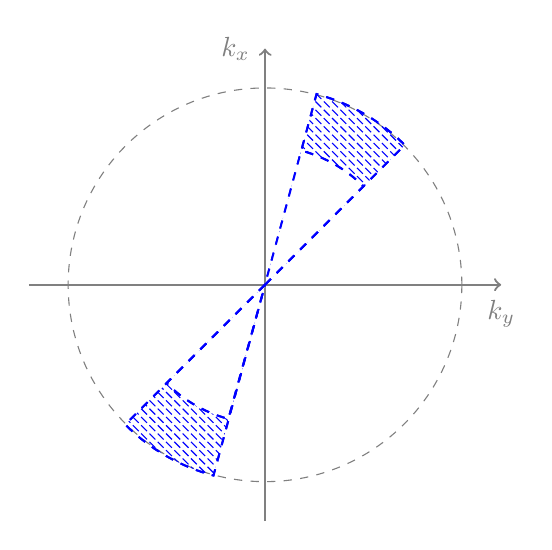
\begin{tikzpicture}
   % Grid
   % \draw [line width=0.5pt, line cap=round, dash pattern=on 0pt off 2\pgflinewidth] (-3,-3) grid (3,3);
    
    Axis
    \draw[thick,->,gray] (-3,0)--(3,0) node[below=1.75pt, fill=white] {$k_y$}; % y axis
    \draw[thick,->,gray] (0,-3)--(0,3) node[left=1.75pt, fill=white] {$k_x$}; % x axis
    
    % Outer Cirlce
    \draw[gray,dashed=onthick] (0,0) circle (2.5cm);

    % -k3 Sector
    \draw[line width=0.25mm,blue,dashed=on 2pt off 3pt, pattern=north west lines, pattern color=blue] (0, 0) -- (-1.775,-1.775) arc[start angle=45 + 180, delta angle=30, radius=2.5cm] -- (0, 0);
    \draw[line width=0.25mm,blue,dashed=on 2pt off 3pt, fill=white] (0, 0) -- (-1.25,-1.25) arc  [start angle=45 + 180, delta angle=30, radius=1.75] -- (0, 0) ;
     \draw[line width=0.25mm,blue,dashed=on 2pt off 3pt] (0, 0) -- (-1.775,-1.775) arc[start angle=45 + 180, delta angle=30, radius=2.5cm] -- (0, 0);
    \draw[line width=0.25mm,blue,dashed=on 2pt off 3pt] (0, 0) -- (-1.25,-1.25) arc  [start angle=45 + 180, delta angle=30, radius=1.75] -- (0, 0) ;
  
    % k3 Sector
    \draw[line width=0.25mm,blue,dashed=on 2pt off 3pt, pattern=north west lines, pattern color=blue] (0,0) -- (1.775,1.775) arc[start angle=45, delta angle=30, radius=2.5cm] -- (0,0);
    \draw[line width=0.25mm,blue,dashed=on 2pt off 3pt, fill=white] (0, 0) -- (1.25,1.25) arc  [start angle=45, delta angle=30, x radius=1.75cm, y radius =1.75cm] ;
    \draw[line width=0.25mm,blue,dashed=on 2pt off 3pt] (0,0) -- (1.775,1.775) arc[start angle=45, delta angle=30, radius=2.5cm] -- (0,0);
    \draw[line width=0.25mm,blue,dashed=on 2pt off 3pt] (0, 0) -- (1.25,1.25) arc  [start angle=45, delta angle=30, x radius=1.75cm, y radius =1.75cm] ;


   \end{tikzpicture}
\end{figure}


Let $\alpha_{\bfkn{1}, \bfkn{2}}^{\bfkn{3}} = \left(k_{1 x} k_{2 y}-k_{2 x} k_{1 y}\right)\left(\frac{1}{\left|\mathbf{k}_{1}\right|^{2}}-\frac{1}{\left|\mathbf{k}_{2}\right|^{2}}\right) a_{\mathbf{k}_{1}} a_{\mathbf{k}_{2}} a_{\mathbf{k}_{3}}$, then we define the following enstrophy flux collective phase for $\mathcal{C}_\theta$

\begin{align}
R_{\mathcal{C}_\theta}\e^{\ii\Phi_{\mathcal{C}_{\theta}}} &= \sum_{\substack{\bfkn{3} \in \mathcal{C}_{\theta} \\ \bfkn{1},  \bfkn{2} \in \mathcal{C}_{\theta}^{'} \\ \bfkn{1} + \bfkn{2} = \bfkn{3}}} \alphakkk{{1}}{2}{3}\e^{\ii \triad{\bfkn{1}}{\bfkn{2}}{\bfkn{3}}} + \sum_{\substack{\bfkn{1}, \bfkn{2} \in \mathcal{C}_{\theta} \\ \bfkn{3} \in \mathcal{C}_{\theta}^{'} \\ \bfkn{1} + \bfkn{2} = \bfkn{3}}} \alphakkk{{1}}{2}{3}\e^{\ii \triad{\bfkn{1}}{\bfkn{2}}{\bfkn{3}}} 
\label{eq:kuramoto_order_param}
\end{align}
where we restrict the summation in the wavevectors to be the right half plane i.e., $k_y > 0$, therefore we only consider the flux into/out of $\mathcal{C}_{\theta}^{+}$. Furthermore the set $\mathcal{C}_{\theta}^{'} \equiv {\mathcal{C}_{\theta}^{+}}^{'}$ can be written as

\begin{align}
	{\mathcal{C}_{\theta}^{+}}^{'} = \bigcup_{\tilde{\theta} \neq \theta} \mathcal{C}_{\tilde{\theta}} \bigcup \mathcal{C}_{\theta}^{L}
\end{align}
where $\mathcal{C}_{\theta}^{L}$ is the lower part of the sector $S_{\theta}$.

Therefore the first term in (\ref{eq:kuramoto_order_param}) becomes

\begin{align}
	\sum_{\substack{\bfkn{3} \in \mathcal{C}_{\theta} \\ \bfkn{1},  \bfkn{2} \in \mathcal{C}_{\theta}^{'} \\ \bfkn{1} + \bfkn{2} = \bfkn{3}}} \alphakkk{{1}}{2}{3}\e^{\ii \triad{\bfkn{1}}{\bfkn{2}}{\bfkn{3}}} &= \sum_{\substack{\bfkn{3} \in \mathcal{C}_{\theta}^{+} \\ \bfkn{1},  \bfkn{2} \in \bigcup_{\tilde{\theta} \neq \theta} \mathcal{C}_{\tilde{\theta}} \bigcup \mathcal{C}_{\theta}^{L} \\ \bfkn{1} + \bfkn{2} = \bfkn{3}}} \alphakkk{{1}}{2}{3}\e^{\ii \triad{\bfkn{1}}{\bfkn{2}}{\bfkn{3}}} \notag \\
	&= \sum_{\tilde{\theta} \neq \theta} \sum_{\substack{\bfkn{3} \in \mathcal{C}_{\theta}^{+} \\ \bfkn{1} \in \mathcal{C}_{\tilde{\theta}} \\ \bfkn{2} \notin \mathcal{C}_{\theta}^{+} \\ \bfkn{1} + \bfkn{2} = \bfkn{3}}} \alphakkk{{1}}{2}{3}\e^{\ii \triad{\bfkn{1}}{\bfkn{2}}{\bfkn{3}}} + \sum_{\substack{\bfkn{3} \in \mathcal{C}_{\theta}^{+} \\ \bfkn{1} \in \mathcal{C}_{\theta}^{L} \\ \bfkn{2} \notin \mathcal{C}_{\theta}^{+} \\ \bfkn{1} + \bfkn{2} = \bfkn{3}}} \alphakkk{{1}}{2}{3}\e^{\ii \triad{\bfkn{1}}{\bfkn{2}}{\bfkn{3}}}
\end{align}

and the second term in (\ref{eq:kuramoto_order_param}) becomes

\begin{align}
	\sum_{\substack{\bfkn{1}, \bfkn{2} \in \mathcal{C}_{\theta} \\ \bfkn{3} \in \mathcal{C}_{\theta}^{'} \\ \bfkn{1} + \bfkn{2} = \bfkn{3}}} \alphakkk{{1}}{2}{3}\e^{\ii \triad{\bfkn{1}}{\bfkn{2}}{\bfkn{3}}} &= \sum_{\substack{\bfkn{1}, \bfkn{2} \in \mathcal{C}_{\theta}^{+} \\ \bfkn{3} \in \bigcup_{\tilde{\theta} \neq \theta} \mathcal{C}_{\tilde{\theta}} \bigcup \mathcal{C}_{\theta}^{L} \\ \bfkn{1} + \bfkn{2} = \bfkn{3}}} \alphakkk{{1}}{2}{3}\e^{\ii \triad{\bfkn{1}}{\bfkn{2}}{\bfkn{3}}} \notag \\
	&= \sum_{\tilde{\theta} \neq \theta} \sum_{\substack{\bfkn{1}, \bfkn{2} \in \mathcal{C}_{\theta}^{+} \\ \bfkn{3} \in \mathcal{C}_{\tilde{\theta}} \\ \bfkn{1} + \bfkn{2} = \bfkn{3}}} \alphakkk{{1}}{2}{3}\e^{\ii \triad{\bfkn{1}}{\bfkn{2}}{\bfkn{3}}} + \sum_{\substack{\bfkn{1}, \bfkn{2} \in \mathcal{C}_{\theta}^{+} \\ \bfkn{3} \in \mathcal{C}_{\theta}^{L} \\ \bfkn{1} + \bfkn{2} = \bfkn{3}}} \alphakkk{{1}}{2}{3}\e^{\ii \triad{\bfkn{1}}{\bfkn{2}}{\bfkn{3}}}
\end{align}

Therefore to obtian the flux into/out of $\mathcal{C}_{\theta}^{+}$ we have

\begin{align}
	\Pi_{\mathcal{C}_{\theta}^{+}} = \sum_{\tilde{\theta} \neq \theta} \left( \sum_{\substack{\bfkn{3} \in \mathcal{C}_{\theta}^{+} \\ \bfkn{1} \in \mathcal{C}_{\tilde{\theta}} \\ \bfkn{2} \notin \mathcal{C}_{\theta}^{+} \\ \bfkn{1} + \bfkn{2} = \bfkn{3}}} \alphakkk{{1}}{2}{3}\e^{\ii \triad{\bfkn{1}}{\bfkn{2}}{\bfkn{3}}} + \sum_{\substack{\bfkn{1}, \bfkn{2} \in \mathcal{C}_{\theta}^{+} \\ \bfkn{3} \in \mathcal{\tilde{\theta}} \\ \bfkn{1} + \bfkn{2} = \bfkn{3}}} \alphakkk{{1}}{2}{3}\e^{\ii \triad{\bfkn{1}}{\bfkn{2}}{\bfkn{3}}} \right) +  \sum_{\substack{\bfkn{3} \in \mathcal{C}_{\theta}^{+} \\ \bfkn{1} \in \mathcal{C}_{\theta}^{L} \\ \bfkn{2} \notin \mathcal{C}_{\theta}^{+} \\ \bfkn{1} + \bfkn{2} = \bfkn{3}}} \alphakkk{{1}}{2}{3}\e^{\ii \triad{\bfkn{1}}{\bfkn{2}}{\bfkn{3}}} + \sum_{\substack{\bfkn{1}, \bfkn{2} \in \mathcal{C}_{\theta}^{+} \\ \bfkn{3} \in \mathcal{C}_{\theta}^{L} \\ \bfkn{1} + \bfkn{2} = \bfkn{3}}} \alphakkk{{1}}{2}{3}\e^{\ii \triad{\bfkn{1}}{\bfkn{2}}{\bfkn{3}}}
\end{align}


which can be loosely interpretted as sum of the contributions to the flux in 1D (along the sector $S_\theta$) and contributions to the flux in 2D which is a function of the angles $\theta$ (denoting the sector that $\bfkn{3}$ lies in) and $\tilde{\theta}$ (the sector that $\bfkn{1}$ lies in)
	
\begin{align}
	\Pi_{\mathcal{C}_{\theta}^{+}} = \sum_{\tilde{\theta} \neq \theta} \Pi_{\text{2D}}(\theta, \tilde{\theta}) + \Pi_{\text{1D}}
\end{align}
and this term can be validated against the flux computed using the nonlinear term of the equations of motion where you consider only the flux contained in the modes in $\mathcal{C}_{\theta}^{+}$

\begin{align}
	\Pi_{\mathcal{C}_{\theta}^{+}} \simeq \der{}{t} \sum_{\bfk \in \mathcal{C}_{\theta}^{+}} |\omega_{\bfk}|^2
\end{align}

\section{Energy Flux}

Using the Fourier vorticity version of the total kinetic energy the rate of change of energy follows in a similar fashion

\begin{align}
	\der{\mathcal{K}}{t} = 2\pi^2\sum_{\bfk}  \frac{1}{|\bfk|^2}\der{a_\bfk^2}{t} =4\pi^2\sum_{\bfk} a_\bfk \frac{\dot{a}_\bfk}{|\bfk|^2}
\end{align}

and 

\begin{align}
	\der{\mathcal{K}}{t} &= 2\pi^2	\sum_{\bfk, \mathbf{k}_1, \mathbf{k}_2\in \mathbb{Z}^2\setminus \mathbf{0}}\left(k_{1x}k_{2y} - k_{1y}k_{2x}\right) \left(\frac{1}{|\bfkn{1}|^2} - \frac{1}{|\bfkn{2}|^2}\right) \left( \frac{1}{|\bfk|^2}\right)a_{\bfkn{1}} a_{\bfkn{2}} a_{\bfk} \cos(\phi_{\bfkn{1}} + \phi_{\bfkn{2}} - \phi_{\bfk})\delta_{\bfkn{1}, \bfkn{2}}^{\bfk} \notag \\ & \qquad \qquad \qquad \qquad- 4\pi^2\nu \sum_{\bfk}|\bfk|^{2p - 2} a_{\bfk}^2 - 4\pi^2\alpha\sum_{\bfk}|\bfk|^{-2q - 2} a_\bfk^2 + 4\pi^2\sum_{\bfk}\frac{a_\bfk}{|\bfk|^2}\Re\left\{\hat{f}_{\bfk} \e^{-\ii\phi_\bfk}\right\}
\end{align}

\section{System Quantities}

\subsection{Enstrophy}

The total Enstrophy for incompressible flows is defined as 

\begin{align}
	\mathcal{E}(\bfu) = \frac{1}{2}\int_{0}^{2\pi} |\curl{\bfu}|^2 \mathrm{d}\bfx \Rightarrow \frac{1}{2}\int_{0}^{2\pi} |\bm{\omega}|^2 \mathrm{d}\bfx = \frac{1}{2}\int_{0}^{2\pi} \omega^2 \mathrm{d}\bfx .
	\label{eq:enstrophy_def}
\end{align}

Using (\ref{eq:fourier_decomp}) the enstrophy in Fourier space is given as 

\begin{align}
	\mathcal{E}(\omegahat{k}) &= \frac{1}{2}\int_{0}^{2\pi} \left(\sum_{\mathbf{k}_1\in \mathbb{Z}^2\setminus \mathbf{0}}\hat{\omega}_{\mathbf{k}_1}\e^{\ii \mathbf{k}_1\cdot \mathbf{x}}\right)\left(\sum_{\mathbf{k}_2\in \mathbb{Z}^2\setminus \mathbf{0}}\hat{\omega}_{\mathbf{k}_2}\e^{\ii \mathbf{k}_2\cdot \mathbf{x}}\right)  \mathrm{d}\bfx, \notag \\
	&= \frac{1}{2}\int_{0}^{2\pi}\sum_{\mathbf{k}_1, \bfkn{2}\in \mathbb{Z}^2\setminus \mathbf{0}}\hat{\omega}_{\mathbf{k}_1}\hat{\omega}_{\mathbf{k}_2} \e^{\ii \left(\mathbf{k}_1 + \bfkn{2}\right)\cdot \mathbf{x}}\mathrm{d}\bfx \notag \\
	&=\frac{1}{2}\sum_{\mathbf{k}_1, \bfkn{2}\in \mathbb{Z}^2\setminus \mathbf{0}}\hat{\omega}_{\mathbf{k}_1}\hat{\omega}_{\mathbf{k}_2} \int_{0}^{2\pi} \e^{\ii \left(\mathbf{k}_1 + \bfkn{2}\right)\cdot \mathbf{x}}\mathrm{d}\bfx \notag \\
	&= \frac{1}{2}\sum_{\mathbf{k}_1, \bfkn{2}\in \mathbb{Z}^2\setminus \mathbf{0}}\hat{\omega}_{\mathbf{k}_1}\hat{\omega}_{\mathbf{k}_2} \delta_{\bfkn{1}, \bfkn{2}} 4 \pi^2 \notag \\
	&= 2 \pi^2 \sum_{\mathbf{k}\in \mathbb{Z}^2\setminus \mathbf{0}}|\hat{\omega}_{\mathbf{k}} |^2 \notag \\
	&= 2 \pi^2 \sum_{\mathbf{k}\in \mathbb{Z}^2\setminus \mathbf{0}} a_{\bfk}^2
	\label{eq:enstrophy_fourier}
\end{align}
where we have let $\bfkn{2} = - \bfkn{1}$ (and relabled as $\bfk$)


\subsection{Kinetic Energy}

The total system energy is defined as

\begin{align}
	\mathcal{K}(\bfu) = \frac{1}{2}\int_0^{2 \pi}|\bfu|^2\mathrm{d}\bfx = \frac{1}{2}\int_0^{2\pi} |(u, v)^{T}|^2 \mathrm{d}\bfx 
\end{align}

Using (\ref{eq:fourier_decomp}) again the total energy in Fourier space becomes

\begin{align}
\mathcal{K}(\hat{u}_{\bfk})	&= \frac{1}{2}\int_0^{2\pi} \left(\sum_{\mathbf{k}_1\in \mathbb{Z}^2\setminus \mathbf{0}}\hat{u}_{\mathbf{k}_1}\e^{\ii \mathbf{k}_1\cdot \mathbf{x}}\right)\left(\sum_{\mathbf{k}_2\in \mathbb{Z}^2\setminus \mathbf{0}}\hat{u}_{\mathbf{k}_2}\e^{\ii \mathbf{k}_2\cdot \mathbf{x}}\right) + \left(\sum_{\mathbf{k}_1\in \mathbb{Z}^2\setminus \mathbf{0}}\hat{v}_{\mathbf{k}_1}\e^{\ii \mathbf{k}_1\cdot \mathbf{x}}\right)\left(\sum_{\mathbf{k}_2\in \mathbb{Z}^2\setminus \mathbf{0}}\hat{v}_{\mathbf{k}_2}\e^{\ii \mathbf{k}_2\cdot \mathbf{x}}\right) \mathrm{d}\bfx \notag\\
	&= \frac{1}{2}\int_0^{2\pi} \sum_{\mathbf{k}_1, \mathbf{k}_2\in \mathbb{Z}^2\setminus \mathbf{0}} (\hat{u}_{\mathbf{k}_1}\hat{u}_{\mathbf{k}_2} + \hat{v}_{\mathbf{k}_1}\hat{v}_{\mathbf{k}_2}) \e^{\ii (\mathbf{k}_1 + \mathbf{k}_2)\cdot \mathbf{x}} \mathrm{d}\bfx \notag \\
	&= \frac{1}{2}\sum_{\mathbf{k}_1, \mathbf{k}_2\in \mathbb{Z}^2\setminus \mathbf{0}} (\hat{u}_{\mathbf{k}_1}\hat{u}_{\mathbf{k}_2} + \hat{v}_{\mathbf{k}_1}\hat{v}_{\mathbf{k}_2}) \int_0^{2\pi} \e^{\ii (\mathbf{k}_1 + \mathbf{k}_2)\cdot \mathbf{x}} \mathrm{d}\bfx \notag \\
	&= \frac{1}{2}\sum_{\mathbf{k}_1, \mathbf{k}_2\in \mathbb{Z}^2\setminus \mathbf{0}} (\hat{u}_{\mathbf{k}_1}\hat{u}_{\mathbf{k}_2} + \hat{v}_{\mathbf{k}_1}\hat{v}_{\mathbf{k}_2}) (2\pi)^2 \delta_{\bfkn{1}, \bfkn{2}} \notag \\
	&= 2\pi^2 \sum_{\mathbf{k}_1\in \mathbb{Z}^2\setminus \mathbf{0}} (\hat{u}_{\mathbf{k}_1}\hat{u}_{-\mathbf{k}_1} + \hat{v}_{\mathbf{k}_1}\hat{v}_{-\mathbf{k}_{1}}) \notag \\
	&= 2\pi^2 \sum_{\mathbf{k}\in \mathbb{Z}^2\setminus \mathbf{0}} (|\hat{u}_{\mathbf{k}}|^2 + |\hat{v}_{\mathbf{k}}|^2)
	\label{eq:energy_u_fourier}
\end{align}
where we have let $\bfkn{2} = - \bfkn{1}$ (and relabled as $\bfk$).

From here we can express the total energy in terms of the vorticity 

\begin{align}
E(\hat{\omega}_{\bfk}) &=  2\pi^2 \sum_{\mathbf{k}\in \mathbb{Z}^2\setminus \mathbf{0}} \left(\left|\mathcal{F}\left[\pder{\psi}{y}\right]_k\right|^2 + \left|\mathcal{F}\left[-\pder{\psi}{x}\right]_k\right|^2 \right) \notag \\
&= 2\pi^2 \sum_{\mathbf{k}\in \mathbb{Z}^2\setminus \mathbf{0}} (|\ii k_{y}\hat{\psi}_{\mathbf{k}}|^2 + |\ii k_x \hat{\psi}_{\mathbf{k}}|^2) \notag \\
&= 2\pi^2 \sum_{\mathbf{k}\in \mathbb{Z}^2\setminus \mathbf{0}} (|\ii k_{y}|^2 + |\ii k_x|^2)|\hat{\psi}_{\mathbf{k}}|^2 \notag \\
&= 2\pi^2 \sum_{\mathbf{k}\in \mathbb{Z}^2\setminus \mathbf{0}} |\bfk|^2\frac{|\hat{\omega}_{\mathbf{k}}|^2}{|\bfk|^4} \notag \\
&= 2\pi^2 \sum_{\mathbf{k}\in \mathbb{Z}^2\setminus \mathbf{0}} \frac{|\hat{\omega}_{\mathbf{k}}|^2}{|\bfk|^2} \notag \\
&= 2\pi^2 \sum_{\mathbf{k}\in \mathbb{Z}^2\setminus \mathbf{0}} \frac{a_{\mathbf{k}}^2}{|\bfk|^2}
\label{eq:energy_w_fourier}
\end{align}

\subsection{Palinstrophy}

 The total palinstrophy is defined as 

 \begin{align}
 \mathcal{P}(\bfu) = \frac{1}{2}\int_0^{2\pi} |\curl{\bm{\omega}}|^2\mathrm{d}\bfx
 \end{align}	
but $\curl{\bm{\omega}} = \grad{\omega}$ in 2D so the palinstrophy is given by

\begin{align}
\mathcal{P}(\bfu) = \frac{1}{2}\int_0^{2\pi} |\grad{\omega}|^2\mathrm{d}\bfx
\end{align}

Using (\ref{eq:fourier_decomp}) again the total palinstrophy in Fourier space becomes

\begin{align}
\mathcal{P}(\omegahat{k}) &= \frac{1}{2}\int_0^{2\pi} \left|\left(\mathcal{F}\left[\pder{\omega}{x}\right]_k, \mathcal{F}\left[\pder{\omega}{y}\right]_k \right)^{T} \right|^2\mathrm{d}\bfx \notag \\
&=  \frac{1}{2}\int_0^{2\pi} \left(\sum_{\mathbf{k}_1\in \mathbb{Z}^2\setminus \mathbf{0}}\ii k_{1x}\hat{\omega}_{\mathbf{k}_1}\e^{\ii \mathbf{k}_1\cdot \mathbf{x}}\right)\left(\sum_{\mathbf{k}_2\in \mathbb{Z}^2\setminus \mathbf{0}}\ii k_{2x}\hat{\omega}_{\mathbf{k}_2}\e^{\ii \mathbf{k}_2\cdot \mathbf{x}}\right) + \left(\sum_{\mathbf{k}_1\in \mathbb{Z}^2\setminus \mathbf{0}}\ii k_{1y}\hat{\omega}_{\mathbf{k}_1}\e^{\ii \mathbf{k}_1\cdot \mathbf{x}}\right)\left(\sum_{\mathbf{k}_2\in \mathbb{Z}^2\setminus \mathbf{0}}\ii k_{2y}\hat{\omega}_{\mathbf{k}_2}\e^{\ii \mathbf{k}_2\cdot \mathbf{x}}\right) \mathrm{d}\bfx \notag\\
&= \frac{1}{2}\int_0^{2\pi} \sum_{\mathbf{k}_1, \mathbf{k}_2\in \mathbb{Z}^2\setminus \mathbf{0}} -(k_{1x}k_{2x} + k_{1y}k_{2y})\hat{\omega}_{\bfkn{1}}\hat{\omega}_{\bfkn{2}}\e^{\ii (\bfkn{1} + \bfkn{2}) \cdot \bfx}\mathrm{d}\bfx \notag\\
&=  \frac{1}{2}\sum_{\mathbf{k}_1, \mathbf{k}_2\in \mathbb{Z}^2\setminus \mathbf{0}} -(k_{1x}k_{2x} + k_{1y}k_{2y})\hat{\omega}_{\bfkn{1}}\hat{\omega}_{\bfkn{2}}\int_0^{2\pi}\e^{\ii (\bfkn{1} + \bfkn{2}) \cdot \bfx}\mathrm{d}\bfx \notag\\
&=  \frac{1}{2}\sum_{\mathbf{k}_1, \mathbf{k}_2\in \mathbb{Z}^2\setminus \mathbf{0}} -(k_{1x}k_{2x} + k_{1y}k_{2y})\hat{\omega}_{\bfkn{1}}\hat{\omega}_{\bfkn{2}} 4\pi^2 \delta_{\bfkn{1}, \bfkn{2}} \notag\\
&=  2\pi^2 \sum_{\mathbf{k}_1, \in \mathbb{Z}^2\setminus \mathbf{0}} -(k_{1x}-k_{1x} + k_{1y}-k_{1y})\hat{\omega}_{\bfkn{1}}\hat{\omega}_{-\bfkn{1}} \notag\\
&=  2\pi^2 \sum_{\mathbf{k}, \in \mathbb{Z}^2\setminus \mathbf{0}} |\bfk|^2 |\hat{\omega}_{\bfk}|^2 \notag\\
&=  2\pi^2 \sum_{\mathbf{k}, \in \mathbb{Z}^2\setminus \mathbf{0}} |\bfk|^2 a_{\bfk}^2 \notag\\
\label{eq:palinstrophy_fourier}
\end{align}


\subsection{Validate System Quantities}

To validate the computation of the system quantities we will compute the various measures for the Taylor Green vortex initial condition which is given by

\begin{align}
u(x, y) &= \kappa\cos(\kappa x)\sin(\kappa y) \notag \\
v(x, y) &= -\kappa\sin(\kappa x)\cos(\kappa y)
\label{eq:taylor_green}
\end{align}
where $\kappa = 1$ 

The total kinetic energy

\begin{align}
\mathcal{K}(\bfu) &= \frac{1}{2}\int_0^{2\pi}|\bfu |^2 \mathrm{d}\bfx \notag \\
									&= \frac{1}{2}\int_0^{2\pi}\left(\cos^2(x)\sin^2(y) + \sin^2(x)\cos^2(y)\right) \mathrm{d}\bfx \notag \\
									&= \frac{1}{2}\int_0^{2\pi}\cos^2(x)\mathrm{d}x\int_0^{2\pi}\sin^2(y)\mathrm{d}y + \frac{1}{2}\int_0^{2\pi}\sin^2(x)\mathrm{d}x\int_0^{2\pi}\cos^2(y)\mathrm{d}y \notag \\
									&= \frac{1}{2}\int_0^{2\pi}\cos^2(x)\mathrm{d}x\int_0^{2\pi}\sin^2(y)\mathrm{d}y + \frac{1}{2}\int_0^{2\pi}\sin^2(x)\mathrm{d}x\int_0^{2\pi}\cos^2(y)\mathrm{d}y \notag \\
									&= \frac{1}{2}\int_0^{2\pi}\frac{\cos(2x) + 1}{2}\mathrm{d}x\int_0^{2\pi}\frac{1 - \cos^2(2x)}{2}\mathrm{d}y + \ldots \notag \\
									&= \frac{1}{2}\left[\frac{\frac{\sin(2x)}{2} + x}{2}\right]_0^{2\pi} \left[\frac{x - \frac{\sin(2x)}{2}}{2}\right]_0^{2\pi} + \ldots  \notag \\
									&= \frac{1}{2}\pi^2 + \frac{1}{2}\pi^2 \notag \\
									&= \pi^2.
\end{align}

The total enstrophy

\begin{align}
\mathcal{E}(\bfu) &= \frac{1}{2}\int_0^{2\pi} |\omega|^2\mathrm{d}\bfx \notag \\
									&= \frac{1}{2}\int_0^{2\pi} \left|\pder{v}{x} - \pder{u}{y}\right|^2 \mathrm{d}\bfx \notag \\
									&= \frac{1}{2}\int_0^{2\pi} |-2 \cos(x)\cos(y)|^2 \mathrm{d}\bfx \notag \\
									&= 2\int_0^{2\pi} \cos^2(x)\cos^2(y) \mathrm{d}\bfx \notag \\
									&= 2\int_0^{2\pi} \cos^2(x)\mathrm{d}x\int_0^{2\pi}\cos^2(y) \mathrm{d}y \notag \\
									&= 2 \pi^2
\end{align}

The total palinstrophy

\begin{align}
\mathcal{P}(\bfu) &= \frac{1}{2}\int_0^{2\pi} |\grad{\omega}|^2 \mathrm{d}\bfx \notag \\
									&= \frac{1}{2}\int_0^{2\pi} |\grad{-2\cos(x)\cos(y)}|^2 \mathrm{d}\bfx \notag \\
									&= \frac{1}{2}\int_0^{2\pi} 4\sin^2(x)\cos^2(y) + 4\cos^2(x)\sin^2(y) \mathrm{d}\bfx \notag \\
									&= 2\int_0^{2\pi} \sin^2(x)\mathrm{d}x\int_0^{2\pi}\cos^2(y)\mathrm{d}y + 2\int_0^{2\pi}\cos^2(x)\mathrm{d}x\int_0^{2\pi}\sin^2(y) \mathrm{d}y \notag \\
									&= 2\pi^2 + 2\pi^2 \notag \\
									&= 4\pi^2
\end{align}

The enstrophy and energy dissipation rates are then $2\nu$ times the palinstrophy and enstrophy respectively.


\end{document}